%% TradeGauntlet paper, arXiv template (arxiv.sty by George Kour, github.com/kourgeorge/arxiv-style).
%% Ported from v2.4 (10 November 2026) by paper/arxiv/make_tex.py. Edit this file directly from now on.
\documentclass{article}

\usepackage{arxiv}

\usepackage[utf8]{inputenc}
\usepackage[T1]{fontenc}
\usepackage{hyperref}
\usepackage{url}
\usepackage{booktabs}
\usepackage{tabularx}
\usepackage{amsfonts}
\usepackage{amsmath}
\usepackage{microtype}
\usepackage{courier}
\usepackage[font=small,skip=6pt]{caption}
\usepackage{graphicx}
\usepackage{xcolor}
\hypersetup{colorlinks=true, linkcolor=black, citecolor=blue!50!black, urlcolor=blue!50!black,
  pdftitle={TradeGauntlet: Testing the Limits of Trading Compliance Controls},
  pdfauthor={Sandip Nandi}}

\title{TradeGauntlet: Testing the Limits of Trading Compliance Controls\\[4pt]
  \large Scripted experiments on order splitting and cancellation timing}
\date{10 November 2026}
\author{Sandip Nandi\\
  Independent Researcher}
\renewcommand{\shorttitle}{TradeGauntlet}
\renewcommand{\headeright}{Preprint}
\renewcommand{\undertitle}{Preprint}

\begin{document}
\maketitle

\begin{abstract}
An order-by-order size limit can admit a large display assembled from smaller orders. We built TradeGauntlet, a custom limit-order-book simulator and replay workflow, to examine this gap while separating alerts, gains from the simulated price response, and costs to legitimate execution. Six 10-lot orders pass the original gate without a conduct alert in all 40 tested seeds. An aggregate cap removes the gain at the original settings, but its effect depends on the assumed response. With throttling disabled, the same 20-lot cap gives a mean responsive-minus-unresponsive wealth difference of 0.00 tick-lots at threshold 0.4 and 48.00 at 0.2. Checks on either side of the response boundary preserve this contrast. The full policy reduces volume by 14.1\% for a large maker and 28.2\% for a patient maker; a separate ablation attributes most of the large maker's loss to throttling. In a one-hour test, submissions resume after lockout but volume remains 75.2\% below the ungated baseline. A legitimate maker triggers alerts in 39/40 episodes at a 170-second quoting interval and 0/40 at 190 seconds, with a 180-second detector window. These scripted cases expose control interactions that can be obscured by reporting alerts alone. The prices are synthetic; the results describe the implemented rules and their consequences, not real-market detection accuracy.
\end{abstract}

\keywords{trading compliance \and market surveillance \and spoofing \and limit order book simulation \and AI trading agents}

\section{Introduction}

A gate may reject a 60-lot order while accepting six 10-lot orders at the same price. Checking each order separately misses the combined display. A cap on total resting quantity addresses that gap, but its usefulness depends on the market response and the legitimate trading it prevents.

Robinhood announced built-in trading agents on September 29, 2026, describing them as coming soon to eligible U.S. customers~\cite{r23}. Its documentation lists order-placement and cancellation tools, with trade approvals on by default and eligible trades allowed without individual confirmation when approvals are disabled~\cite{r24}. This raises a practical question: how should orders be supervised once an agent has permission to trade? Our experiments evaluate scripted controls, without using Robinhood software or customer data.

We built TradeGauntlet for this study: a small limit-order-book simulator coupled to a workflow for fixing scenarios, comparing controls on matched paths, and replaying the resulting orders. We distinguish whether a surveillance rule flags a sequence, whether a gate removes its gain from the simulated price response, and how much legitimate execution the gate prevents. An alert records a pattern; a rejection records an intervention. Neither alone tells us whether the intervention removed the gain or whether the trading was lawful.

The experiments vary the aggregate cap and price-response threshold together, then examine cancellation windows and session lengths. A further test changes a legitimate maker's quoting interval relative to the detector window. These comparisons expose three problems: protection that depends on the assumed response, recovery that leaves substantial execution costs, and alerts on ordinary quoting. Each can be missed if an evaluation reports only alerts or rejected orders.

The contribution is a set of executable counterexamples and a workflow for retesting them after a control change. The simulator makes the rule interactions inspectable; it does not estimate how often they occur in markets. All reported trading actions come from fixed scripts. Section 9 describes the pending extension to LLM agents.

\section{Related work}

Wang and Wellman~\cite{r1} study spoofing with trading agents, and Wang et al.~\cite{r7} extend the analysis to strategic responses and market-design changes. Cartea, Jaimungal, and Wang~\cite{r18} model the trade-off between spoofing gains and expected fines. These studies explain economic mechanisms that our fixed scripts and imposed price response take as given.

Tao et al.~\cite{r19} derive spoofing conditions from a multilevel imbalance model, calibrate it to TMX Level-2 data, and propose monitoring based on distributional distance. Chen, Hsieh, and Yang~\cite{r20} use Taiwan derivatives order and trade data to study potential spoofing and a price-banding intervention. Both bring market evidence to questions of detection or trading restrictions. Here the response model is uncalibrated, so the comparisons measure effects within the simulator.

Two working papers address evidence that this design lacks. Do and Putni\c{n}\v{s}~\cite{r13} evaluate indicators using prosecuted cases and out-of-sample tests. Fabre and Challet~\cite{r10} use Level-3 data to estimate price responses and possible spoofing gains. External labels and an estimated response would strengthen our evaluation; varying an assumed threshold does not supply either.

Learning traders can adapt to detection and enforcement. Byrd~\cite{r2} studies an RL trader that discovers spoofing and a learned recognizer that discourages it. Wang and Wellman~\cite{r3} model adaptation between manipulation and detection, while Cartea, Chang, and Garc\'{i}a-Arenas~\cite{r12} examine manipulation by learning algorithms. Gu et al.~\cite{r17} vary liquidity and spoofing strategies, and ABIDES~\cite{r4} supports richer agent interaction and communication latency. We hold the trading policies fixed to isolate the effects of control settings.

Pandey and Rajwal~\cite{r25} evaluate LLM judgments about potential market abuse using variants of enforcement-case narratives. RISCTrade~\cite{r26} evaluates adherence to risk mandates during trading across multiple markets. We focus on what happens at the order level when a gate or surveillance rule changes, including the cost to legitimate execution.

InvestorBench~\cite{r27} compares LLM agents across financial tasks and assets. FinAgent~\cite{r28} develops a multimodal trading agent with tools and memory. QFinZero~\cite{r29} provides standardized financial tools, stateful brokerage simulation, order-lifecycle management, and replay. Here, we compare interacting controls on matched market paths. Testing how an LLM adapts to those controls remains future work.

ReguSim~\cite{r8} separates a trader's reasoning, attempted orders, enforcement, and monitoring evidence; its reported environment uses exogenous prices and fully executes accepted orders. Borjigin and He~\cite{r9} propose constrained execution with a runtime shield, leaving the full cryptographic proof pipeline for future work. Kurshan, Balch, and Byrd~\cite{r5} discuss agent-based governance, and Byrd~\cite{r11} studies trading with LLM-generated social posts. Our experiments contain neither model-selected trades nor a social-information channel.

\section{TradeGauntlet: simulator, gates, and detectors}

\subsection{Market mechanics}

TradeGauntlet uses a custom matching engine, implemented for this project, with integer prices, price/time priority, and partial fills. It is not built on ABIDES. Scenario runners fix the configuration and random seeds, execute paired control conditions, record attempted and accepted actions, and replay saved attempts to check event hashes and outcomes. Cap multiples, response thresholds, throttle windows, session lengths, and quoting cadences can be varied through these runners. Orders execute within the simulator, with no broker or exchange connection; this is what offline means here.

\begin{table}[htbp]
\centering
\small
\begin{tabularx}{\linewidth}{lX}
\toprule
\textbf{Component} & \textbf{Specification} \\
\midrule
Book and matching & One evaluated account and one instrument; integer ticks, price/time priority, partial fills \\
Timing & One second per attempted action; background replenishment every second; default decisions every 60 seconds, with exact re-quote times in the cadence boundary checks \\
Background liquidity & Three price levels per side, 10 lots per level, centered around the fundamental plus any response \\
Exogenous path & Fundamental starts at 1,000; increments -1, 0, +1 with probabilities 1/4, 1/2, 1/4 every 30 seconds; noise quantities 0, 1, 2 with probabilities 1/2, 1/4, 1/4 every 10 seconds \\
Risk and fees & 100-lot worst-case position commitment; fee 0.05 tick-lots per filled lot \\
Sessions & 720 seconds in the core study; 720 and 3,600 seconds in the throttle tests; no warm-up \\
\bottomrule
\end{tabularx}
\end{table}

The fundamental and noise streams are generated before trading starts. For a given seed and session length, every gate and response condition therefore receives the same exogenous draws. Unfilled market quantity expires. Background quotes are replaced between successive subject actions, so splitting an order also changes how long the display remains in the book.

Immediately before each replenishment, let B and A be total remaining buy and sell quantity, including the subject. The imbalance is I = (B - A) / max(1, B + A). In the responsive condition, background quotes shift by two ticks when I exceeds a threshold t, by minus two ticks when I is below -t, and otherwise do not shift. The unresponsive condition omits this shift. The original threshold is 0.4; the sensitivity grid varies it. This step response is stipulated, not estimated from market data.

\subsection{Pre-trade gates}

All conditions enforce the position-commitment bound. The legacy gate additionally rejects a limit submission above twice external reference depth, more than two resting price levels on a side, and a predicted self-match. Reference depth is the median external quantity at the two touches, excluding subject orders. The aggregate gate adds a per-side cap: remaining subject limit quantity plus the full proposed quantity must not exceed m times reference depth. Originally m = 2. The sensitivity grid varies this aggregate multiple while retaining the legacy per-order multiple of 2.

Both gates can throttle new limit and market submissions when C/N > 0.9 and N is at least 20, where C and N count subject cancellations and accepted submissions in the trailing window. The original window is 1,800 seconds. Rejected attempts do not increase N; cancellations remain available. Throttle-off conditions make the minimum submission count unreachable, without changing other gate checks. The aggregate check runs at submission and does not rebalance existing orders as external depth changes. It also checks a marketable limit at its full submitted quantity, so its rejection cost is intentionally conservative.

\subsection{Pattern definitions}

For a canceled order i, let q\textsubscript{i} be submitted quantity, d\textsubscript{i} its submission-time external reference depth, and a\textsubscript{i} its age at cancellation. Let h\textsubscript{i} be the fraction of q\textsubscript{i} filled before cancellation and z\textsubscript{i} its distance from the same-side touch at submission. For a subject fill f on the opposite side, define Q(i,f) to hold when i was nonmarketable at submission, submission precedes f, f precedes cancellation, a\textsubscript{i} is at most W, and h\textsubscript{i} < 0.1. Event sequence numbers determine ordering within a timestamp. The implemented rules are:

\begin{table}[htbp]
\centering
\small
\begin{tabularx}{\linewidth}{lX}
\toprule
\textbf{Signal} & \textbf{Condition for an alert} \\
\midrule
Individual pattern & Some i and f satisfy Q(i,f), q\textsubscript{i} $\geq$ 3d\textsubscript{i}, and z\textsubscript{i} $\leq$ 3 ticks. \\
Layer pattern & For one f and one displayed side, qualifying Q(i,f) orders occupy at least three distinct prices. No individual-size or distance test is added. \\
Aggregate pattern & For one f and displayed side, at least two Q(i,f) orders have z\textsubscript{i} $\leq$ 3 and positive remaining quantity r\textsubscript{i}(f). Their sum is at least 3 times the maximum d\textsubscript{i} in that group. \\
Self-match & The subject is both buyer and seller in a fill. \\
\bottomrule
\end{tabularx}
\end{table}

Remaining quantity r\textsubscript{i}(f) is measured immediately before the shared fill, after any earlier partial executions. The conduct-alert union contains these four signals; a separate cancellation-ratio diagnostic is excluded. The current scoring default is W = 180 seconds, shared by the individual, layer, and aggregate patterns. Table 2 retains the original 120-second configuration to document the initial split-order comparison; the cadence grid varies W explicitly. These patterns do not implement a complete legal test or estimate trader intent.

\section{Comparisons and experimental design}

Terminal wealth is cash plus inventory valued at the terminal fundamental, after fees. For gate g, parameters p, and seed s, the response-dependent difference is D(g,p,s) = W(responsive,g,p,s) - W(unresponsive,g,p,s). The two conditions use the same gate and exogenous path. Positive D indicates a benefit from this particular response toggle; it is not a legal or general welfare measure. Executed lots, rejected actions by reason, and response activations are reported separately.

The split probe alternates sides. Each cycle submits six 10-lot orders at one price, executes two lots on the opposite side, and cancels the surviving display. The legitimate controls are small and large two-sided makers, a patient maker, a passive scheduled executor, and a 10-lot slice executor. We assign these scripts their objectives; the assignments have not been independently reviewed. The scheduled executor is named \texttt{vwap\_executor} in the code, but uses neither a volume forecast nor a VWAP benchmark.

Core comparisons use 40 seeds per arm. The cadence study reuses 40 paths across quoting intervals and detector windows. A parameter sample varies order count, total quantity, price spread, submission gaps, lifetime overlap, and execution delay. Each of the original 40 draws was paired with one market seed, and the same draws were used to tune the detector window. Those results describe performance on the tuning cases, not held-out recall.

\begin{table}[htbp]
\centering
\small
\begin{tabularx}{\linewidth}{lXr}
\toprule
\textbf{Sensitivity analysis} & \textbf{Conditions} & \textbf{Episodes} \\
\midrule
Cap and response & 2 scripts x 6 response thresholds x (ungated + 5 aggregate caps) x 10 seeds x 2 response states & 1,440 \\
Parameter replication & 12 new vectors from the existing generator x 5 market seeds x 2 thresholds x 2 gates x 2 response states & 480 \\
Throttle and horizon & 2 session lengths x (ungated + 2 gates x 4 windows + 2 gates without throttle) x 10 seeds & 220 \\
Price boundaries & 3 cap multiples x 2 neighboring thresholds x 2 scripts x 2 gates x 10 seeds x 2 response states & 480 \\
Cadence boundaries & 170- and 190-second maker cadences x 40 ungated seeds; scored at W = 180 & 80 \\
\bottomrule
\end{tabularx}
\caption{Sensitivity and boundary checks: 2,700 episodes. The first three comparisons contain 2,140 episodes; the boundary checks add 560. The cap grid uses m in \{1, 2, 3, 4, 6\} and t in \{0.1, 0.2, 0.25, 0.3, 0.4, 0.5\}. Neighboring thresholds are 0.24/0.26 at m = 2, 0.39/0.41 at m = 4, and 0.49/0.51 at m = 6. Cap and parameter comparisons disable throttling. The horizon study uses t = 0.4, m = 2, and throttle windows of 120, 300, 900, and 1,800 seconds.}
\end{table}

The settings and parameter vectors were saved before each comparison was run, after inspecting the earlier results. This is exploratory analysis, not preregistration. Seeds 8000-8009 pair the cap and price-boundary conditions, 8100-8104 pair each parameter vector, and 8200-8209 pair the horizon conditions. Cadence checks reuse seeds 6000-6039. The runners are \texttt{paper\_study.sensitivity} and \texttt{paper\_study.boundary}. Tables give means with observed minimum and maximum values; these ranges are descriptive, not confidence intervals. Reused paths, rescoring, and parameter draws from one authored generator do not supply independent strategy samples.

\section{Aggregation and the price-response boundary}

\begin{table}[htbp]
\centering
\small
\begin{tabular}{lllll}
\toprule
\textbf{Gate} & \textbf{Original alerts} & \textbf{With aggregate signal} & \textbf{Executed lots} & \textbf{Wealth} \\
\midrule
off & 0/40 & 40/40 & 24.00 [24.00, 24.00] & 22.05 [14.80, 32.80] \\
legacy & 0/40 & 40/40 & 24.00 [24.00, 24.00] & 22.05 [14.80, 32.80] \\
aggregate & 0/40 & 0/40 & 24.00 [24.00, 24.00] & -25.95 [-33.20, -15.20] \\
\bottomrule
\end{tabular}
\caption{Six-by-ten split probe, \texttt{pilot.review\_study}, seeds 3000-3039, responsive market. Both gates include the original throttle. The 120-second scoring window is retained from this comparison; rescoring at the current 180-second default leaves these alert counts unchanged. Alerts count episodes; volume and wealth are mean [minimum, maximum]. Wealth is in tick-lots.}
\end{table}

Each split order passes the individual-size check, and all occupy one price level. The individual and layer detectors flag none of these 40 paths; the aggregate detector flags the admitted sequence. Under the aggregate gate, however, absence of an aggregate alert is guaranteed for fixed m < 3. At admission of the last qualifying order j, the group's quantity cannot exceed m d\textsubscript{j}. Its remaining quantity at the shared fill can only decrease, so its sum is at most m max\textsubscript{i} d\textsubscript{i}, below the detector's 3 max\textsubscript{i} d\textsubscript{i} threshold. This assumes every group order passed the same gate and cannot increase in size after admission. The zero count at m = 2 therefore says nothing about independent detector accuracy.

The original settings make this result structurally likely. With three intact background levels of D lots per side and subject display mD on only one side, I = m/(6 + m). Thus m = 2 gives I = 0.25, below 0.4. Under these static assumptions, activation requires m > 6t/(1 - t); at t = 0.4, the boundary is m = 4. Trades can deplete depth before replenishment, so 0.25 is not a global bound on the simulated book. A replay diagnostic of the 40 gated parameter draws nevertheless finds no response activations and a maximum absolute imbalance of 0.282. Their identical responsive and unresponsive event streams therefore verify a restricted mechanism, not general economic prevention.

\begin{figure}[htbp]
\centering
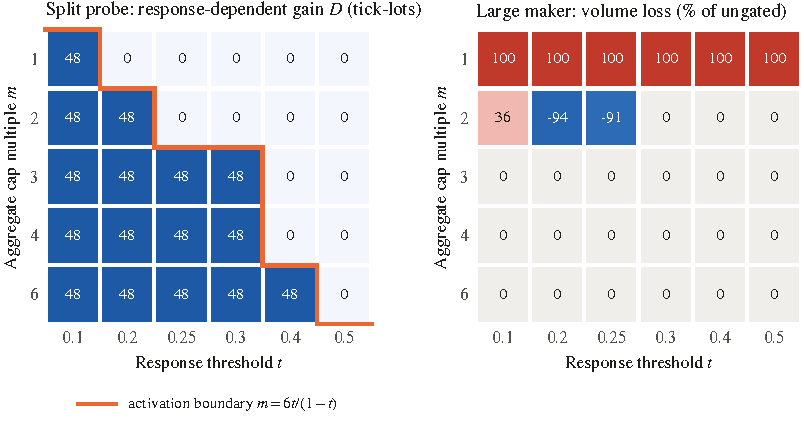
\includegraphics[width=\linewidth]{figures/cap_response.pdf}
\caption{Cap-response sensitivity with throttling disabled. Left: mean D for the split probe, in tick-lots; each cell has zero spread across its ten seeds. Right: loss of mean large-maker volume relative to the ungated mean at the same threshold; negative values mean higher gated volume. The ungated arms are the baselines and are not separate plotted rows. Only the aggregate cap varies; the individual limit stays twice reference depth.}
\end{figure}

At the original 20-lot aggregate cap, mean D is 0.00 at t = 0.4 and 48.00 at t = 0.2, positive on 10/10 paired paths. All split-probe cells in Figure 1 follow the static response boundary. The equalities (m,t) = (2,0.25), (4,0.4), and (6,0.5) give zero because activation uses a strict inequality. At the neighboring thresholds in Table 1, each lower-threshold cell gives D = 48 on every seed, and each upper cell gives D = 0. The contrast thus persists away from equality, while remaining a consequence of the imposed response. At m = 1, all 12-lot maker quotes exceed the allowance: the maker executes nothing, a 100\% volume loss.

\begin{table}[htbp]
\centering
\small
\begin{tabular}{lllll}
\toprule
\textbf{Threshold} & \textbf{Gate} & \textbf{D: mean [min, max]} & \textbf{D > 0} & \textbf{D > 0, no alert} \\
\midrule
0.2 & off & 16.47 [-5.25, 50.80] & 44/60 & 5/60 \\
0.2 & aggregate & 10.96 [-5.85, 65.90] & 30/60 & 30/60 \\
0.4 & off & 11.32 [0.00, 50.80] & 27/60 & 0/60 \\
0.4 & aggregate & 0.00 [0.00, 0.00] & 0/60 & 0/60 \\
\bottomrule
\end{tabular}
\caption{Parameter replication, \texttt{paper\_study.sensitivity}: 12 vectors crossed with seeds 8100-8104, cap multiple 2, throttle disabled, W = 180 seconds. D is mean [minimum, maximum] in tick-lots. Each denominator is 60 draw-seed pairs, not 60 independent strategies. Positive D remains counted even if other actions were rejected.}
\end{table}

At threshold 0.2, 30/60 gated draw-seed pairs retain a positive response-dependent wealth difference without a conduct alert. At threshold 0.4, the same cap leaves no positive differences. The throttle is disabled in both comparisons, so these results isolate response sensitivity. The 48 tick-lots in Figure 1 also follow from the stipulated mechanism: 12 cycles times two executed lots times a two-tick response when every execution benefits. The sweep checks this dependence; it does not estimate a response from market data.

At cap multiple 2 and response thresholds 0.2 and 0.25, the gate with its throttle disabled increases maker volume. Changing the display changes the subsequent book response and fills, so accepting fewer orders need not reduce execution. Higher volume alone says little about execution quality. Additional paths test sensitivity within the same strategy generator; smooth responses, varying liquidity, queue calibration, and strategic background traders remain untested.

\section{Throttle timing and legitimate trading cost}

The cancellation throttle counts accepted submissions, so the number of quotes admitted per decision affects when it starts. In \texttt{pilot.throttle\_isolation}, seeds 4000-4039, removing only the aggregate gate's throttle raises mean volume from 50.93 to 59.05 lots, close to 59.48 ungated. Thus most of the large maker's loss in that matched comparison comes from throttling. Its 720-second session is shorter than the 1,800-second window, so a triggered lockout cannot expire during trading. The horizon experiment below uses a separate seed cohort; its baselines should not be substituted for those in this ablation or Table 5.

\begin{figure}[htbp]
\centering
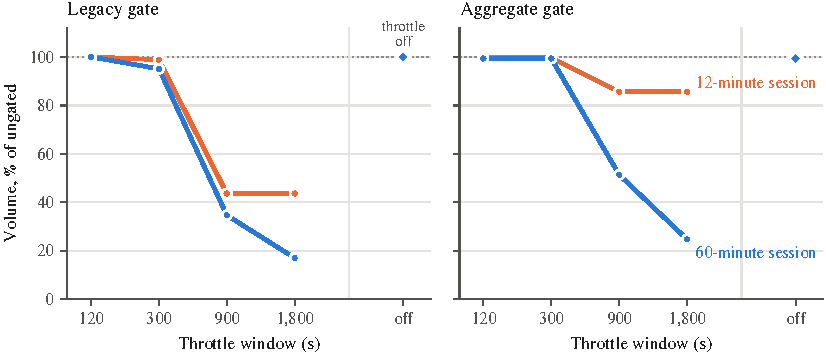
\includegraphics[width=\linewidth]{figures/throttle_horizon.pdf}
\caption{Mean volume as a percentage of the ungated mean at the same horizon, \texttt{paper\_study.sensitivity}, seeds 8200-8209. Lines join finite throttle windows; separate diamonds disable only the throttle. Percentages are ratios of means. Panels distinguish the legacy and aggregate policies.}
\end{figure}

\begin{table}[htbp]
\centering
\small
\begin{tabular}{llllll}
\toprule
\textbf{Minutes} & \textbf{Gate} & \textbf{Executed lots} & \textbf{Throttle rejects} & \textbf{Throttled} & \textbf{Recovered} \\
\midrule
12 & off & 60.50 [34.00, 90.00] & 0.00 [0, 0] & 0/10 & 0/10 \\
12 & legacy & 26.40 [13.00, 59.00] & 26.80 [16, 28] & 10/10 & 0/10 \\
12 & aggregate & 51.80 [29.00, 90.00] & 6.80 [0, 8] & 9/10 & 0/10 \\
60 & off & 300.60 [263.00, 355.00] & 0.00 [0, 0] & 0/10 & 0/10 \\
60 & legacy & 51.20 [31.00, 74.00] & 197.50 [188, 200] & 10/10 & 10/10 \\
60 & aggregate & 74.40 [38.00, 210.00] & 169.40 [97, 180] & 10/10 & 10/10 \\
\bottomrule
\end{tabular}
\caption{Large maker from \texttt{pilot.revision}, run by \texttt{paper\_study.sensitivity} on seeds 8200-8209. Gates use a 1,800-second throttle window; off is the matched ungated baseline. Lots and throttle rejects are mean [minimum, maximum]. The last columns count episodes. Recovered means at least one accepted submission after the first throttle rejection, not uninterrupted trading.}
\end{table}

In the one-hour condition, all ten aggregate-gated episodes resume submissions after a throttle rejection. Mean volume is nevertheless 74.40 lots, compared with 300.60 ungated: a 75.2\% loss. The short-session aggregate arm averages 51.80 against 60.50 lots. Extending the session reveals recovery, but also repeated periods in which the maker cannot submit orders.

Session length determines whether recovery can be observed. The trailing window, quoting rate, and minimum submission count determine whether throttling starts and how often it recurs. A short window can keep the count below the trigger altogether. A longer session can allow submissions to resume while still losing substantial volume. These settings must be assessed together; the tests do not select an optimal throttle for a live market.

\setcounter{table}{4}\renewcommand{\thetable}{5a}

\begin{table}[htbp]
\centering
\small
\begin{tabular}{llll}
\toprule
\textbf{Legitimate task} & \textbf{Ungated lots} & \textbf{Aggregate lots} & \textbf{Volume loss} \\
\midrule
Scheduled executor & 27.38 [11.00, 50.00] & 27.38 [11.00, 50.00] & 0.0\% \\
10-lot slice executor & 30.12 [12.00, 45.00] & 30.12 [12.00, 45.00] & 0.0\% \\
Small maker & 31.05 [20.00, 36.00] & 31.05 [20.00, 36.00] & 0.0\% \\
Large maker & 56.50 [33.00, 88.00] & 48.55 [27.00, 87.00] & 14.1\% \\
Patient maker, 300 s & 66.28 [32.00, 109.00] & 47.60 [30.00, 69.00] & 28.2\% \\
\bottomrule
\end{tabular}
\caption{Full aggregate policy, including the 1,800-second throttle, versus no policy gate in 720-second sessions. Volume is mean [minimum, maximum] over seeds 6000-6039; loss is a ratio of means. The strategies are defined in \texttt{pilot.negative\_controls}. These paths differ from the throttle-isolation and horizon cohorts.}
\end{table}

\renewcommand{\thetable}{\arabic{table}}

\setcounter{table}{4}\renewcommand{\thetable}{5b}

\begin{table}[htbp]
\centering
\small
\begin{tabular}{lllll}
\toprule
\textbf{Legitimate task} & \textbf{Size cap} & \textbf{Throttle} & \textbf{Position} & \textbf{Other} \\
\midrule
Scheduled executor & 0.00 [0, 0] & 0.00 [0, 0] & 0.00 [0, 0] & 0.00 [0, 0] \\
10-lot slice executor & 0.00 [0, 0] & 0.00 [0, 0] & 0.00 [0, 0] & 0.00 [0, 0] \\
Small maker & 0.00 [0, 0] & 0.00 [0, 0] & 0.00 [0, 0] & 0.00 [0, 0] \\
Large maker & 20.30 [20, 24] & 7.40 [0, 8] & 0.00 [0, 0] & 0.25 [0, 2] \\
Patient maker, 300 s & 6.00 [6, 6] & 0.00 [0, 0] & 0.00 [0, 0] & 0.03 [0, 1] \\
\bottomrule
\end{tabular}
\caption{Rejected actions under the same aggregate policy: mean [minimum, maximum]. Size cap combines individual and aggregate size checks; every size rejection here is aggregate. Other comprises cancellation attempts on inactive orders. Each attempt records only its first failed check, so counts reconcile but do not causally apportion lost volume.}
\end{table}

\renewcommand{\thetable}{\arabic{table}}

The large maker loses 14.1\% of volume in Table 5a. Its 27.95 mean rejections comprise 20.30 size-cap rejections, 7.40 throttle rejections, and 0.25 failed cancellations. The separate throttle ablation shows why rejection counts alone cannot attribute the volume loss. The patient maker loses 28.2\% without any throttle rejections; its cost arises under the remaining gate checks. The passive scheduled and slice executors receive no gate rejections, yet complete only 34.2\% and 37.7\% of their 80-lot parent orders. These are task-completion measurements, not operational false-rejection rates or full best-execution assessments.

\section{Detector timing and legitimate counterexamples}

The age condition in Q(i,f) excludes orders canceled after W, whatever their purpose. Moving a maker's quoting interval across W changes which orders are eligible for an alert. The shared fill, remaining quantity, and other conditions in Section 3.3 must still hold.

\begin{figure}[htbp]
\centering
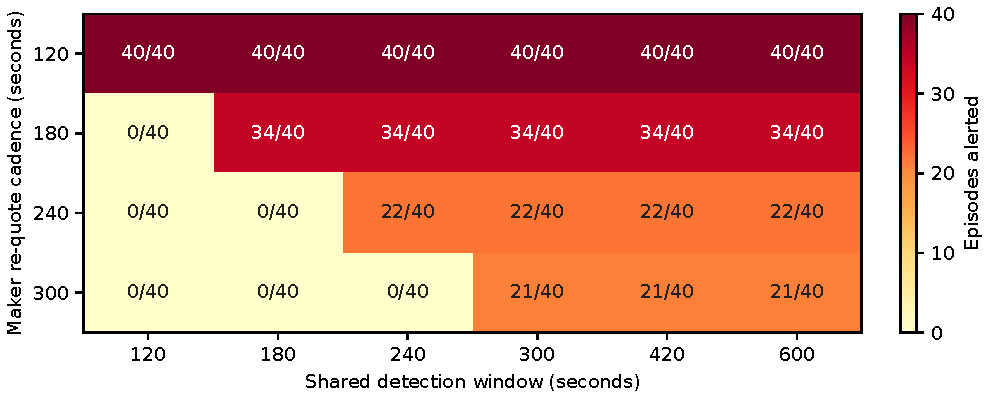
\includegraphics[width=\linewidth]{figures/cadence.pdf}
\caption{Rule-boundary check on an authored legitimate maker. Counts show conduct alerts among 40 ungated episodes at each cadence and shared scoring window. Each row uses the same seed cohort; each trajectory is rescored across windows. The staircase follows the rule's age condition and is not a measured operational false-positive curve.}
\end{figure}

At W = 180 seconds, the 180-second maker alerts in 34/40 episodes and the 300-second maker in none. The rule includes equality: a\textsubscript{i} $\leq$ W. Exact-time checks at 170 and 190 seconds give 39/40 and 0/40 alerts, respectively, on the same seeds. The scheduler reproduces all 40 original 180-second event hashes before these checks. Thus a legitimate quoting schedule also triggers alerts strictly inside the window. The staircase remains a property of the age condition, not an empirical false-positive curve.

We selected and assessed the original window on the same cases. Extending W from 120 to 180 seconds raised detections from 10/15 to 15/15 selected economic cases, so the improvement is tuning performance rather than independent recall. The choice of legitimate controls matters as well. A buy-only executor cannot meet the opposite-side-own-fill condition, and a small maker cannot challenge the aggregate size threshold. Controls outside the rule's eligible region provide little evidence about its specificity within that region.

For the 180-second maker, the aggregate policy reduces mean volume from 73.80 to 58.98 lots and produces no conduct alerts. The gate has changed the activity available to the detector. The disappearance of alerts, alongside reduced execution, does not establish better discrimination. Evaluating specificity beyond these examples requires separate strategy families and independently reviewed objectives.

\section{Practical use and regulatory context}

TradeGauntlet can be used to rerun a trading task and market path after a change to a cap, throttle, or scoring window. The saved configuration, attempted actions, rejection reasons, and event hashes allow a developer to trace a change in fills or alerts to the control setting. The examples show why this matters: zero alerts can be enforced by a size inequality, a recovered throttle can still suppress trading, and ordinary quoting can match a detector pattern. Reuse requires choosing cases that challenge the proposed control; passing the existing scripts is not a deployment criterion.

An agent may react to a rejected order by changing its next decision. That reaction is absent from a replay of fixed actions. Studying it requires fresh model decisions in each control condition and separate records of attempted orders, accepted orders, alerts, and task outcomes. Such an experiment would complement the market-abuse judgment and risk-mandate studies~\cite{r25,r26} by examining adaptation to these order-level controls.

For FINRA member firms, these tests relate to the technical controls used in market-conduct supervision. Rule 3110~\cite{r15} concerns the supervisory system and responsibilities. Notice 15-09~\cite{r14} discusses algorithm development, change control, testing, monitoring, and records, and recommends testing independently of development. Our experiment was developed and assessed within the same project. It does not provide that independent validation or assess a firm's supervisory organization.

FINRA Rule 5210.03~\cite{r16} includes a Type 1 disruptive-quoting pattern with multiple price levels, a supply-and-demand change, opposite-side trading, and withdrawal. The layering script resembles parts of that sequence; the same-price split probe does not reproduce the multiple-level condition. The single-account self-match check also falls short of the beneficial-ownership and related-algorithm considerations in Rule 5210.02. Notice 24-09~\cite{r6} applies existing obligations to generative-AI use; it provides context for the proposed agent study, not evidence that these scripts evaluate AI supervision.

In the U.S. derivatives context, the CFTC's guidance on CEA section 4c(a)(5)(C) makes intent to cancel before execution material and distinguishes legitimate good-faith cancellation~\cite{r21}. An order pattern or an author-assigned script label cannot establish that legal intent. This framework and FINRA supervision address different regulatory settings; the simulator is not a jurisdiction-specific compliance test.

EU RTS 6 provides a further testing connection~\cite{r22}. Articles 5 and 7 address development and testing methodology and separation of testing from production. Article 13 addresses surveillance adequacy, false alerts, and replay of order and transaction data. These provisions motivate examining both suspicious sequences and legitimate activity. Our logs and simulations do not demonstrate fulfillment of the regulation's organizational, surveillance, or recordkeeping obligations.

The size multiples, cancellation ratios, and time windows are experimental choices, not regulatory thresholds. An alert still needs interpretation, and an accepted sequence is not a certification of compliance.

\section{Limitations and the agent study}

The model has one evaluated account, one instrument, three replenishing levels, and a two-tick step response. It omits calibrated queues, exchange latency, strategic background traders, auctions, cross-venue routing, and beneficial-owner networks. Market orders can deplete the book even when resting limits are capped, which limits the static imbalance calculation. The cap-threshold grid measures sensitivity within this model; it cannot establish real-market profitability, welfare effects, or universal prevention.

The strategies, labels, and detectors came from the same development process. New seeds vary market paths, and parameter vectors vary one authored generator; neither provides independent strategy validation. The detector window was tuned on earlier cases. Sensitivity and boundary settings were then selected in response to observed results. The resulting means and ranges describe these exploratory comparisons, with no population-level accuracy or power claim.

Even the one-hour sessions are short and synthetic. A single accepted submission after a rejection counts as recovery, although further lockouts may follow. Executed volume also leaves out inventory risk, adverse selection, opportunity cost, and other aspects of execution quality. The gate conservatively checks the full quantity of a marketable limit order and can reject an executable order. Its measured costs belong to that implementation.

The planned LLM study will assign legitimate execution and market-making tasks, then compare order patterns and task completion under different controls. Models, prompts, tools, failure handling, and analysis must be fixed before evaluation. Repeated model calls on one market path are not independent market scenarios. Internally authored holdouts would need to be supplemented by externally authored cases, independent behavior review, and market calibration before making stronger generalization claims. The LLM results remain pending.

\section{Conclusion and availability}

An aggregate limit closes the illustrated order-splitting gap, but whether it removes the trading gain depends on the assumed price response. Execution costs depend on both the size cap and the cancellation throttle; alert counts can also be fixed by inequalities shared with the gate. Ordinary market making provides a further counterexample when its quoting interval falls inside the detector window. TradeGauntlet records these interactions as replayable tests, with alerts, response-dependent gains, and legitimate execution assessed separately. Calibrated markets, independently designed strategies, and adaptive LLM traders remain to be tested.

\subsection{Code and data availability}

Code, saved results, and reproduction instructions: \href{https://github.com/tokencraftdata/agentic-compliance/tree/f92f3260686e9da2a8da6bbe3be064d07487a8e2}{github.com/tokencraftdata/agentic-compliance}. The repository is currently private.

\subsection{Use of generative AI tools}

Anthropic Claude Code assisted with the throttle-isolation, parameterized-evasion, negative-control, and detector-window-sweep modules, their tests, and results notes. OpenAI Codex assisted with the matched-counterfactual, cadence-grid, and sensitivity studies, the paper builder, literature checks, and manuscript drafting and revision. These tools were used to produce the research artifact; the reported trading experiments used fixed scripts and made no LLM calls. The human author is responsible for the methods, results, and references.

\small

\begin{thebibliography}{99}

\bibitem{r1} Xintong Wang and Michael P. Wellman. Spoofing the Limit Order Book: An Agent-Based Model. AAMAS, 2017, pp. 651-659.
\url{https://www.ifaamas.org/Proceedings/aamas2017/pdfs/p651.pdf}

\bibitem{r2} David Byrd. Learning Not to Spoof. Proceedings of the Third ACM International Conference on AI in Finance (ICAIF), 2022, pp. 139-147.
\url{https://doi.org/10.1145/3533271.3561767}

\bibitem{r3} Xintong Wang and Michael P. Wellman. Market Manipulation: An Adversarial Learning Framework for Detection and Evasion. IJCAI, 2020, pp. 4626-4632.
\url{https://doi.org/10.24963/ijcai.2020/638}

\bibitem{r4} David Byrd, Maria Hybinette, and Tucker Hybinette Balch. ABIDES: Towards High-Fidelity Multi-Agent Market Simulation. Proceedings of the 2020 ACM SIGSIM Conference on Principles of Advanced Discrete Simulation, 2020, pp. 11-22.
\url{https://doi.org/10.1145/3384441.3395986}

\bibitem{r5} Eren Kurshan, Tucker Balch, and David Byrd. The Agentic Regulator: Risks for AI in Finance and a Proposed Agent-based Framework for Governance. arXiv:2512.11933, 2025.
\url{https://arxiv.org/abs/2512.11933}

\bibitem{r6} FINRA. Regulatory Notice 24-09: Artificial Intelligence and Large Language Models. June 27, 2024.
\url{https://www.finra.org/rules-guidance/notices/24-09}

\bibitem{r7} Xintong Wang, Christopher Hoang, Yevgeniy Vorobeychik, and Michael P. Wellman. Spoofing the Limit Order Book: A Strategic Agent-Based Analysis. Games 12(2), 46, 2021.
\url{https://doi.org/10.3390/g12020046}

\bibitem{r8} Yiyang Luo et al. ReguSim: Evaluating LLM Agent Rule Grounding in Financial Compliance. arXiv:2608.19974, version 2, 2026.
\url{https://arxiv.org/abs/2608.19974v2}

\bibitem{r9} Ailiya Borjigin and Cong He. Safe and Compliant Cross-Market Trade Execution via Constrained RL and Zero-Knowledge Audits. arXiv:2510.04952, version 2, 2025.
\url{https://arxiv.org/abs/2510.04952v2}

\bibitem{r10} Timoth\'{e}e Fabre and Damien Challet. Learning the Spoofability of Limit Order Books With Interpretable Probabilistic Neural Networks. arXiv:2504.15908, 2025.
\url{https://arxiv.org/abs/2504.15908}

\bibitem{r11} David Byrd. The Accidental Pump and Dump: When Agentic AI Meets Autonomous Trading. ICAIF, 2025, pp. 88-95.
\url{https://doi.org/10.1145/3768292.3770424}

\bibitem{r12} \'{A}lvaro Cartea, Patrick Chang, and Gabriel Garc\'{i}a-Arenas. Spoofing and Manipulating Order Books with Learning Algorithms. SSRN 4639959, 2023; revised February 17, 2025.
\url{https://doi.org/10.2139/ssrn.4639959}

\bibitem{r13} Bao Linh Do and T\={a}lis J. Putni\c{n}\v{s}. Detecting Layering and Spoofing in Markets. SSRN 4525036, 2023.
\url{https://doi.org/10.2139/ssrn.4525036}

\bibitem{r14} FINRA. Regulatory Notice 15-09: Guidance on Effective Supervision and Control Practices for Firms Engaging in Algorithmic Trading Strategies. March 26, 2015.
\url{https://www.finra.org/rules-guidance/notices/15-09}

\bibitem{r15} FINRA. Rule 3110: Supervision. Rulebook, accessed November 9, 2026.
\url{https://www.finra.org/rules-guidance/rulebooks/finra-rules/3110}

\bibitem{r16} FINRA. Rule 5210: Publication of Transactions and Quotations, including Supplementary Material .02 and .03. Rulebook, accessed November 9, 2026.
\url{https://www.finra.org/rules-guidance/rulebooks/finra-rules/5210}

\bibitem{r17} Anri Gu et al. The Effect of Liquidity on the Spoofability of Financial Markets. ICAIF, 2024, pp. 239-247.
\url{https://doi.org/10.1145/3677052.3698634}

\bibitem{r18} \'{A}lvaro Cartea, Sebastian Jaimungal, and Yixuan Wang. Spoofing and Price Manipulation in Order-Driven Markets. Applied Mathematical Finance 27(1-2), 2020, pp. 67-98.
\url{https://doi.org/10.1080/1350486X.2020.1726783}

\bibitem{r19} Xuan Tao, Andrew Day, Lan Ling, and Samuel Drapeau. On detecting spoofing strategies in high-frequency trading. Quantitative Finance 22(8), 2022, pp. 1405-1425.
\url{https://doi.org/10.1080/14697688.2022.2059390}

\bibitem{r20} Jianqiang Chen, Pei-Fang Hsieh, and J. Jimmy Yang. Order spoofing, price impact, and market quality. Pacific-Basin Finance Journal 97, 2026, article 103077.
\url{https://doi.org/10.1016/j.pacfin.2026.103077}

\bibitem{r21} Commodity Futures Trading Commission. Antidisruptive Practices Authority: Interpretive guidance and policy statement. Federal Register 78, 2013, pp. 31890-31897.
\url{https://www.cftc.gov/LawRegulation/FederalRegister/FinalRules/2013-12365.html}

\bibitem{r22} European Commission. Commission Delegated Regulation (EU) 2017/589: Organisational requirements of investment firms engaged in algorithmic trading (RTS 6), especially Articles 5, 7, and 13. Official Journal L 87, 2017, pp. 417-448.
\url{https://eur-lex.europa.eu/eli/reg_del/2017/589/oj/eng}

\bibitem{r23} Robinhood. Robinhood Puts the Power of Hedge Funds in Every Trader's Pocket. Company announcement, September 29, 2026. Accessed November 10, 2026.
\url{https://robinhood.com/newsroom/hood-summit-2026/}

\bibitem{r24} Robinhood. Trading with your agent. Product documentation, accessed November 10, 2026.
\url{https://robinhood.com/us/en/support/articles/trading-with-your-agent/}

\bibitem{r25} Avinash Kumar Pandey and Swati Rajwal. Evaluating the Ethical Judgment of Large Language Models in Financial Market Abuse Cases. Proceedings of the 6th ACM International Conference on AI in Finance (ICAIF), 2025, pp. 132-140.
\url{https://doi.org/10.1145/3768292.3770439}

\bibitem{r26} Wenliang Huang, Junkai Li, Zengyi Yu, and Xiangjie Kong. RISCTrade: A Dynamic Multi-Market Benchmark for Risk-Mandate Compliance of Large Language Models in Closed-Loop Trading. Advanced Intelligent Computing Technology and Applications (ICIC 2026), LNCS 16648, Springer, 2027, pp. 360-370. First online July 14, 2026.
\url{https://doi.org/10.1007/978-981-92-3400-4_30}

\bibitem{r27} Haohang Li et al. INVESTORBENCH: A Benchmark for Financial Decision-Making Tasks with LLM-based Agent. Proceedings of ACL 2025, Volume 1: Long Papers, pp. 2509-2525.
\url{https://doi.org/10.18653/v1/2025.acl-long.126}

\bibitem{r28} Wentao Zhang et al. A Multimodal Foundation Agent for Financial Trading: Tool-Augmented, Diversified, and Generalist. Proceedings of the 30th ACM SIGKDD Conference on Knowledge Discovery and Data Mining (KDD), 2024.
\url{https://doi.org/10.1145/3637528.3671801}

\bibitem{r29} Haochen Luo et al. QFinZero: A Unified Financial Toolchain for LLM-Based Trading Agents. Proceedings of ACL 2026, Volume 3: System Demonstrations, pp. 68-77.
\url{https://doi.org/10.18653/v1/2026.acl-demo.7}

\end{thebibliography}

\end{document}
